\documentclass[a4paper]{article}
\usepackage{graphicx}
\usepackage{twocolpceurws}
\usepackage{float}
\usepackage{hyperref}
\usepackage{todonotes}
\usepackage{tikz}
\def\checkmark{\tikz\fill[scale=0.4](0,.35) -- (.25,0) -- (1,.7) -- (.25,.15) -- cycle;} 

\title{Towards Automated Merging of Code Clones in Object-Oriented Programming Languages\\- Work in Progress -}

\author{
Simon Baars \\ University of Amsterdam\\
                Amsterdam, Netherlands \\ simon.mailadres@gmail.com
\and
Ana Oprescu \\ University of Amsterdam\\
                Amsterdam, Netherlands \\
                AM.Oprescu@uva.nl
}

\institution{}

\begin{document}
\maketitle

\begin{abstract}
Duplication in source code can have a major negative impact on the maintainability of source code, as it creates explicit dependencies between fragments of code. Such explicit dependencies often cause bugs. In this study, we look into the opportunities to automatically refactor these duplication problems for object-oriented programming languages. To do this, we propose a method to detect clones that are suitable for refactoring. This method focuses on the context and scope of clones, ensuring our refactoring improves the design and does not leave side effects after it is applied.

Our intermediate results indicate that more than half of the duplication in code is related to each other through inheritance, making it easier to refactor these clones in a clean way. Approximately a fifth of the duplication can be refactored through method extraction, while other clones require other refactoring techniques. Similar future measurements will provide further insight into the contexts where clones occur and how this affects the automated refactoring process. Finally, we strive to construct a tool that automatically applies refactorings for a large part of the detected duplication problems.
\end{abstract}

\section{Introduction}
Duplication in source code is often seen as one of the most harmful types of technical debt. In Martin Fowler's ``Refactoring'' book \cite{fowler1999refactoring}, he claims that \textit{``Number one in the stink parade is duplicated code. If you see the same code structure in more than one place, you can be sure that your program will be better if you find a way to unify them.''}. 
% In this research, we take a look at the challenges and opportunities in automatically refactoring duplicated code, also known as ``code clones''. The main goal is to improve the maintainability of the refactored code.

Refactoring is used to improve the quality-related attributes of a codebase (maintainability, performance, etc.) without changing the functionality. Many methods were introduced to aid the process of refactoring~\cite{fowler1999refactoring, wake2004refactoring}, and are integrated into most modern IDE's. However, most of these methods still require a manual assessment of where and when to apply them. This means refactoring is either a significant part of the development process~\cite{lientz1978characteristics, mens2004survey}, or does not happen at all~\cite{mens2003refactoring}. For a large part, proper refactoring requires domain knowledge. However, there are also refactoring opportunities that are rather trivial and repetitive to execute. In this research, we investigate the extent to which code clones can be automatically refactored.

A survey by Roy et al. \cite{roy2007survey} describes different types of clones. Most clone detection tools focus on finding clones corresponding with these definitions. In this paper, we outline challenges with these clone type definitions when considered in a refactoring context. We next propose solutions to these problems that would enable the detection of clones that should be refactored, rather than fragments of code that are just similar. 

Code clones can be found anywhere in a codebase. The location of a clone in the code has an impact on how it can be refactored. Therefore, we first look at where and how often clones can be found, enabling the prioritization of refactoring opportunities.
% Using this information we can determine in which locations clones are found the most, on basis of which the refactoring will be prioritized. 

Furthermore, a duplicate fragment in a codebase does not always have to be an exact match with another fragment to be considered a clone. Therefore, we also analyze the impact of the different definitions of clone types on refactoring opportunities.
% We look at the definitions of different types of clones and the opportunities to refactor duplicate parts of code albeit not an exact match. 

We conduct our research on a large corpus of open source projects. We focus mainly on the Java programming language as refactoring opportunities feature paradigm and programming language dependent aspects~\cite{choi2011extracting}. However, most practices featured in this research will also be applicable to other object-oriented languages, like C\#.

In this research, we strive to improve upon the current state-of-the-art in clone refactoring \cite{fontana2015duplicated, alwaqfi2017refactoring} by building a clone refactoring tool that automatically applies refactorings to a large percentage of clones found. The design decisions for this tool are made on basis of data gathered from a large corpus of software systems. 

Section 

\section{Background}\label{chap:background}
As code clones are seen as one of the most harmful types of technical debt, they have been studied extensively. A survey by Roy et al.~\cite{roy2007survey} states definitions of important concepts in code clone research. For instance, ``clone pair''is defined as \textit{a set of two code portions/fragments which are identical or similar to each other}; ``clone class'' as \textit{the union of all clone pairs}; ``clone instance'' as a single code portion/fragment that is part of either a clone pair or clone class.
\subsection{Advantages of clone classes over clone pairs}\label{chap:cloneclasses}
Regarding clone detection, there is a lot of variability in literature whether clone pairs or clone classes should be detected. In this study we focus on clone classes, because of the advantages for refactoring. Clone pairs don not provide a general overview of all entities containing the clones, with all their related issues and characteristics \cite{fontana2012duplicated}. Although clone classes are harder to manage, they provide all information needed to plan a suitable refactoring strategy, since this way all instances of a clone are considered. Another issue involves clone grouping by pairs: single clone reference amount increases according to binomial coefficient formula (two clones form a pair, three clones form three pairs, four clones form six pairs, and so on), of which a heavy information redundancy follows \cite{fontana2012duplicated}.

\subsection{Clone types}
In a 2007 survey by Roy et al. \cite{roy2007survey} he defines four types of clones:\\
\textbf{Type 1:} Identical code fragments except for variations in whitespace (may be also variations in layout) and comments.\\
\textbf{Type 2:} Structurally/syntactically identical fragments except for variations in identifiers, literals, types, layout and comments.\\
\textbf{Type 3:} Copied fragments with further modifications. Statements can be changed, added or removed in addition to variations in identifiers, literals, types, layout, and comments.\\
\textbf{Type 4:} Two or more code fragments that perform the same computation but implemented through different syntactic variants.

A higher type of clone means that it is harder to detect. It also makes the clone harder to refactor, as more transformations would be required. Higher clone types also become more disputable whether they actually indicate a harmful antipattern (as not every clone is harmful \cite{jarzabek2010clones, kapser2008cloning}).
\subsection{Related work in clone refactoring tools}
The Duplicated Code Refactoring Advisor (DCRA) looks into refactoring opportunities for clone pairs \cite{fontana2012duplicated, fontana2015duplicated}. This tool only focuses on refactoring clone pairs, the authors arguing that \textit{clone pairs are much easier to manage when considered singularly.} As intermediate steps, the authors measure a corpus of Java systems for some clone-related properties of the systems, like the relation (in terms of inheritance) between code fragments in a clone pair.
 
Aries \cite{higo2004aries, higo2008metric} focuses on the detection of refactoring oriented clones. On basis of the relation between clone instances through inheritance, similar to Fontana et al. \cite{fontana2012duplicated}, Aries proposes a refactoring. For instance, if two clone classes are siblings of each other (share the same superclass), they propose to perform ``Extract method'' and ``Pull up method'' sequentially. This tool only proposes such a refactoring, and does not provide help in the process of applying the refactoring.

There are many other research efforts looking into code clone refactoring \cite{alwaqfi2017refactoring, chen2018clone, koni2001scenario}. However, all of these tools only support a subset of all harmful clones that are found. Also, these tools are limited to suggesting refactoring opportunities, rather than actually applying refactorings where suitable. Finally, all published approaches have limitations, such as false positives in their clone detection \cite{chen2018clone} or being limited to clone pairs \cite{higo2008metric}.

\section{Clone Detection}\label{chap:clonedetection}
As duplication in source code is a serious problem in many software systems, many research efforts look into code clones. Many tools have been proposed to detect various types of code clones. Two surveys of modern clone detection tools \cite{sheneamer2016survey, svajlenko2014evaluating} together show an overview of the most-popular clone detection tools up until 2016. \todo{what is insufficient about these two? what triggered the need to reassess clone detectors? where are the four criteria coming from?}

\subsection{Survey on Clone Detection Tools}
\label{ch:tool-overview}
We conducted a short survey on (recent) clone detection tools that we could use to analyze refactoring possibilities. The results of our survey are displayed in table~\ref{table:dettools}. We chose a set of tools that are open source and can analyze either Java or Python. Then we chose four criteria by which we considered these tools: 
\begin{enumerate}
    \item \textbf{Should find clones in any context.} We want to perform an analysis on a set of projects. In this analysis we want to be able to get a full overview of cloning in the set of projects. Some tools only find clones in specific contexts, like only method-level clones. Because of that, we want to use a clone detection tool that is able to find clones in any context.
\item \textbf{Should detect clone classes in a number of example projects.} We have created a number of test projects\footnote{Our test projects to assess the validity of clone detection tools: \url{https://github.com/SimonBaars/CloneRefactor/tree/master/src/test/resources}} that we used to assess the validity of clone detection tools. On basis of this, we checked whether clone detection tools can correctly find clones in diverse contexts.
\item \textbf{Considers dependency graphs to be sure that this clone can be merged.} When detecting clones for refactoring purposes, it is important that clone instances are actually equal. Sometimes, to verify actual equality (not just textual equality), it is required to consider resolved symbols (this is described more elaborately in section \ref{chap:type1clones}). Because of this, we want to use a clone detection tool that can analyze such structures.
\item \textbf{Makes it possible to configure the way in which clones are detected (as in what to exclude from the detection) in a relatively straightforward way.} We aim to exclude expressions/statements from matching (more about our rationale in section~\ref{chap:clonetypes}). To achieve this, the tool needs to be able to recognize the meaning of certain tokens.
\end{enumerate}

\begin{table}[H]
 \begin{center}
  \caption{Our survey on clone detection tools.} \label{table:dettools}
  \bigskip
\begin{tabular}{|l|l|l|l|l|l|}
\hline
\textbf{Clone Detection Tool} & \textbf{(1)} & \textbf{(2)} & \textbf{(3)} & \textbf{(4)} \\ \hline
Siamese \cite{ragkhitwetsagul2019siamese} &  &             &             & \checkmark            \\ \hline
NiCAD \cite{roy2008nicad, cordy2011nicad} \footnote{}           & \checkmark                             & \checkmark            &             &             \\ \hline
CPD \cite{roy2009comparison}\footnote{} & \checkmark & \checkmark            &             &             \\ \hline
\begin{tabular}[c]{@{}l@{}}CCFinder \cite{kamiya2002ccfinder}\\ CCFinderX\\ D-CCFinder \cite{livieri2007very}\end{tabular} & \checkmark  & \checkmark   &    &   \\ \hline
CCFinderSW \cite{semura2017ccfindersw}   & \checkmark     &             &             & \checkmark            \\ \hline
\begin{tabular}[c]{@{}l@{}}SourcererCC \cite{sajnani2016sourcerercc}\\ Oreo \cite{saini2018oreo}\end{tabular} & \checkmark    &             &             & \checkmark            \\ \hline
BigCloneEval \cite{svajlenko2016bigcloneeval}  & \checkmark  & \checkmark   &             &             \\ \hline
Deckard \cite{jiang2007deckard} & \checkmark   &             & \checkmark            &             \\ \hline
\end{tabular}
\end{center}
\end{table}

\footnotetext[3]{This clone detection tool has also been used by Fontana et al. \cite{fontana2012duplicated}}
\footnotetext{\label{note1}CPD is a Clone Detection tool that is part of PMD. PMD is a widely used tool for static code analysis in Java.}

None of the tools we considered implement all our criteria, so we decided to implement our own clone detection tool: CloneRefactor\footnote{CloneRefactor (WIP) is available on GitHub: \url{https://github.com/SimonBaars/CloneRefactor}}.



\subsection{CloneRefactor}
A 2016 survey by Gautam \cite{gautam2016various} focuses more on various techniques for clone detection. We decided to combine AST- and Graph-based approaches for clone detection, similar to Scorpio \cite{higo2013revisiting, kamalpriya2017enhancing}. However, instead of building a dependency graph, we build a similarity graph of statements linking to similar statements. The graph built by CloneRefactor is shown in figure \ref{fig:clonerefactor}. 

We decided to base our tool on the JavaParser library \cite{tomassetti2017javaparser}, as it supports rewriting the AST back to Java code and is compatible with all modern Java versions (Java 1-12). We collect each statement and declaration and compare those to find duplicates. This way we build a graph of each statement/declaration linking to each subsequent statement/declaration (horizontally) and linking to each of its duplicates (vertically). On basis of this graph we detect clone classes.

We challenge completed clone classes against the thresholds that are being used, and remove the clone classes that do not adhere to the thresholds.
 
\begin{figure}[H]
  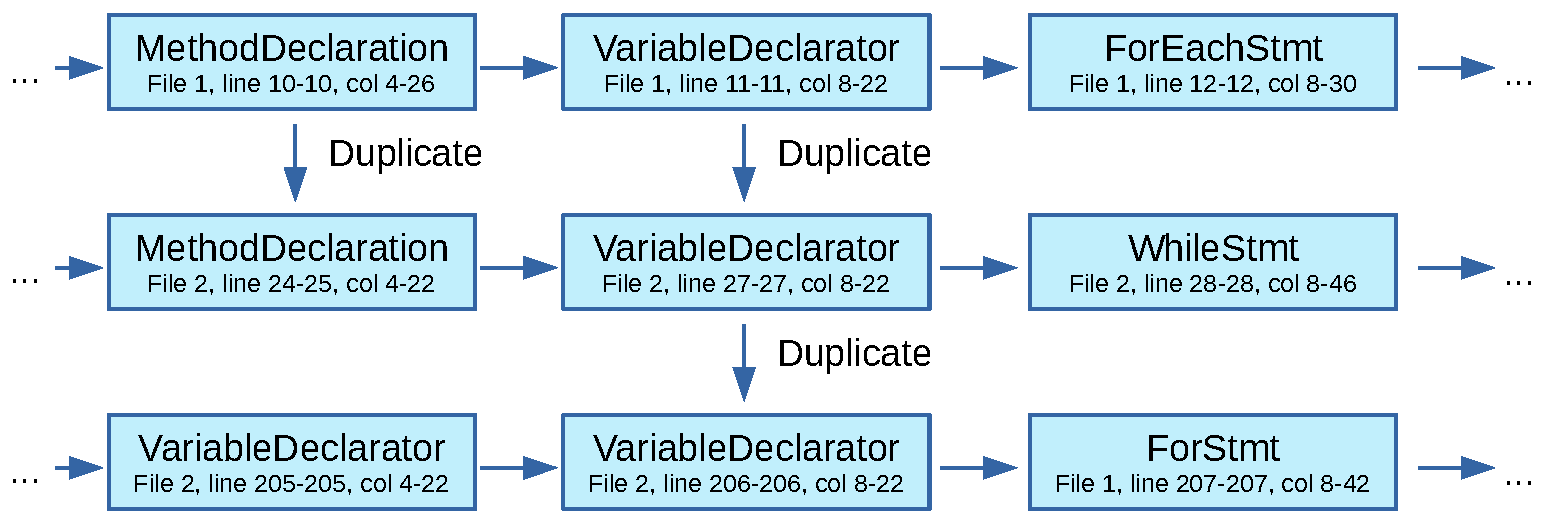
\includegraphics[width=1\columnwidth]{img/CodeGraph}
  \caption{Abstract figure of the graph representation built by CloneRefactor}
  \label{fig:clonerefactor}
\end{figure}

\subsubsection{Thresholds}\label{chap:thresholds}
CloneRefactor works on basis of three thresholds for finding clones:
\begin{enumerate}
  \item \textbf{Number of statements/declarations:} The number of statements/declarations that should be equal/similar for it to be considered a clone.
  \item \textbf{Number of tokens:} The number of tokens (excluding whitespace, end-of-line terminators and comments) that should be equal/similar for it to be considered a clone.
  \item \textbf{Number of lines:} The minimum amount of lines (excluding lines that do not contain any tokens, for tokens same exclusions apply) that should be equal/similar for it to be considered a clone.
\end{enumerate}
Of course, if any threshold is set to zero, it will be ignored, thus not all thresholds have to be used at all times. We consider ``number of lines'' to be the least important, as it highly depends on the programmer of the codebase (and we do not want this kind of dependence!). On basis of manual assessment, we have determined that setting the ``number of statements/declarations'' to 6 ensures that most non-harmful clones are filtered out. On the downside, this also filters out some harmful antipatterns. For instance, if a cloned statement has many tokens we might want to consider it a clone even if it spans less than 6 statements (as a cloned line with many tokens is more harmful than one with few).

The measurements in our study use the following thresholds:
\begin{itemize}
  \item \textbf{Number of statements/declarations:} 6
  \item \textbf{Number of tokens:} 10
  \item \textbf{Number of lines:} 6
\end{itemize}

\section{Addressing problems with clone type definitions}\label{chap:clonetypes}
We propose solutions for shortcomings in type 1, type 2 and type 3 clones~\cite{roy2007survey} to increase the chance that we can merge the clone while improving the design. Due to the serious challenges involved in their detection and refactoring, type 4 clones are not considered in this study.

\subsection{Type 1 clones} \label{chap:type1clones}
Type 1 clones are identical clone fragments except for variations in whitespace and comments. However, when two clone fragments are textually identical, it does not yet indicate that they are actually identical. Even when textually equal, method calls can refer to different methods, type declarations can refer to different types and even variables can be of a different type. This could invalidate a refactoring opportunity for such a code fragment. Therefore, we propose to:
\begin{itemize}
  \item \textbf{Compare the equality of the fully qualified method signature for method references.} If an identifier is fully qualified, it means we specify the full location of its declaration (e.g. \texttt{com.simonbaars.fruitgame.Apple} for an \texttt{Apple} object). This way we can validate whether two method references, like method calls, are actually equal. In the method signature, not only the fully qualified identifier of the method should be considered, but also the type of all its arguments. This way we can be sure that two potentially cloned method references do not point to overloaded variants (in a case that the data type of arguments is overloaded).
  \item \textbf{Compare the equality of the fully qualified identifier for type references.} This way we can be sure that two referenced types are actually equal, and that they are not just two types with the same name.
  \item \textbf{Compare the equality the fully qualified identifier for variable usages.} Two cloned lines might use a variable with the same name, but different types. This might pose serious challenges on refactoring, as the variables might not concern the same object or primitive. To check this, we need to track the declaration of variables and from this infer the fully qualified identifier of its type.
\end{itemize}

\subsection{Type 2 clones}
By definition, type 2 clones allow any change in identifiers, literals, types, layout, and comments. For refactoring purposes, this does not always make a lot of sense. If we allow any change in identifiers, literals, and types, we cannot distinguish between different variables, different types and different method calls anymore. This could render two methods that have an entirely different functionality as clones. Merging such clones might only prove to be harmful.

We tackle these problems with type 2 clones to be able to detect such clones that can and should be merged. Our definition ensures functional similarity by applying the following changes to type 2 clones:

\begin{itemize}
  \item \textbf{Considering types:} The definition of type 2 clones states that types should not be considered. We disagree because types can make a significant change to the meaning of a code segment and thus whether this segment should be considered a clone.
  \item \textbf{Having a distinction between different variables:} By the definition of type 2 clones, any identifiers would not be taken into account. We agree that a difference in identifiers may still result in a harmful clone, but we should still consider the distinction between different variables. For instance, if we call a method like this: \texttt{myMethod(var1, var2)}, or call this method like this: \texttt{myMethod(var1, var1)}. Even if the variables have the same type, the distinction between the variables is important to ensure the functionality is the same after merging.
  \item \textbf{Defining a threshold for variability in literals:} By the definition of type 2 clones any literals would not be taken into account. We agree, as when merging the clone (for instance by extracting a method), we can simply turn the literal into a method parameter. However, we would argue that thresholds matter here. How many literals may differ for the segment still to be considered a clone with another segment? We need to define a threshold to be sure that, by merging, we are not replacing a code fragment by a worse maintainable design.
  \item \textbf{Consider method call signatures and define a threshold for variability in method calls:} As type-2 clones allow changes in identifiers, also the names of called methods may vary. However, because of this, completely different methods can be called in cloned fragments as a result. This poses serious challenges on refactoring and makes it more disputable whether such a clone is actually harmful. This is because different method identifiers can describe a completely different functionality. Therefore, we suggest considering the call signatures of cloned methods when they are compared. We can allow variability in the rest of method identifiers by passing the function as a parameter. To limit the amount of parameters required we also recommend defining a threshold for variability in method call expressions, so only a limited number of method calls can vary.
\end{itemize}

\subsection{Type 3 clones}
Type 3 clones are even more permissive than type 2 clones, allowing added and removed statements. Thresholds matter a lot here to make sure that not the whole project is detected as a clone of itself. The main question for this study regarding type 3 clones is: ``how can we merge type 3 clones while improving the design?''.

Clone instances in type 3 clones are almost always different in functionality. As we have to ensure equal functionality after merging the clone, we have to wrap the difference in statements between the clone instances in conditional blocks (either if-statements or switch-statements). We can then pass a variable as to which path should be taken through the code (either a boolean or an enumeration). Such a refactoring would make added statements that are contiguous less harmful for the design than added statements that are separated by statements that both clone instances have in common.

We also argue that statements that are not common between two clone instances, should not count towards the size of the clone (and thus towards the threshold which determines whether the clone will be taken into account). Also, clones should not start and not end with an added statement (as that would be nonsense: such a thing could be done for any clone).

As for the detection of type 3 clones, we think the easiest opportunity to detect these clones is to consider it as a postprocessing step after clone detection. By trying to find short gaps between clones, we can find opportunities to merge clone classes into a single type 3 clone class. The amount of statements that this ``short gap'' can maximally span should be dependent on a threshold value.

\section{Relation, Location and Content Analysis of Clones}\label{chap:clonecontextexpl}
To be able to refactor code clones, it is very important to consider the context of the clone. We define the following aspects of the clone as its context:
\begin{enumerate}
  \item The relation of clone instances among each other through inheritance (for example: a clone instance resides in a superclass of another clone instance in the same clone class).
  \item Where a clone instance occurs in the code (for example: a method-level clone is a clone instance that is in a method).
  \item The contents of a clone instance (for example: the clone instance spans several methods).
\end{enumerate}
Figure \ref{fig:clonecontext} shows an abstract representation of clone classes and clone instances. The relation of clones through inheritance is measured on clone class level: it involves all child clone instances. The location and contents of clones is measured on clone instance level. A clone's location involves the file it resides in and the range it spans (for example: line 6 col 2 - line 7 col 50). A clone instance contents consists of a list of all statements and declarations it spans.
\begin{figure}[H]
    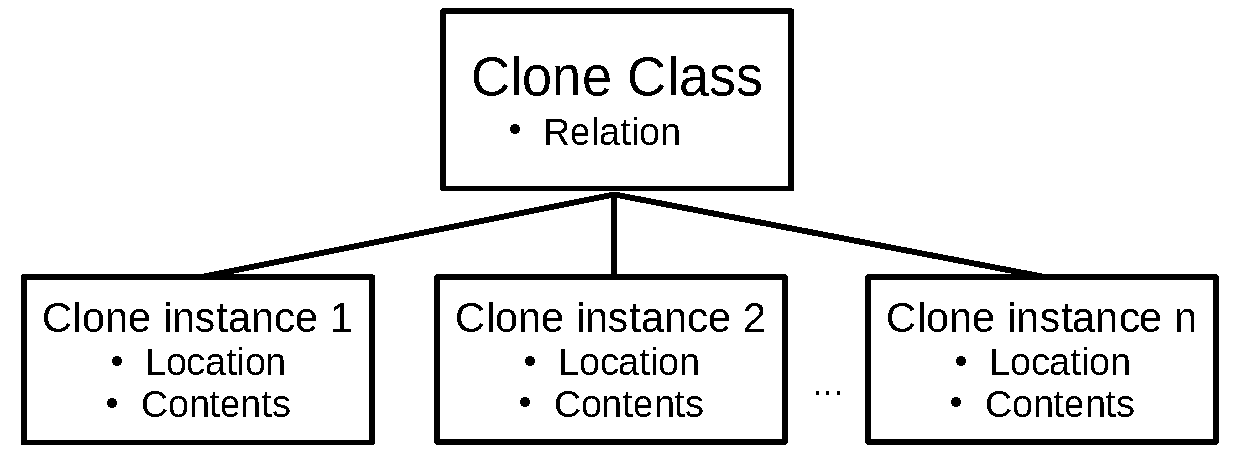
\includegraphics[width=1\columnwidth]{img/context}
  \caption{Abstract representation of clone classes and clone instances.}
  \label{fig:clonecontext}
\end{figure}
%\todo{do we have proof of this statement? if not, say that this is our intuition and a first step to prove it is to analyze a large body of projects} Everything in the context of a clone has a big impact on how it has to be refactored. 
% I guess it's a bit of an empty statement. Of course where some code is located has an impact on how to refactor it. Maybe remove it?
We analyzed the context of clones in a large corpus of open source projects. For these experiments, we used the CloneRefactor tool. These experiments map the context, as follows: the relation between clone instances is explained, measured and discussed in section\ref{chap:relationsinstances}; the location of clone instances is explained, measured and discussed in section \ref{chap:clonelocation};  the content of clone instances are explained, measured and discussed in section \ref{chap:clonecontents}.

\subsection{The corpus}\label{chap:corpus}
For our measurements we use a large corpus of open source projects \cite{githubCorpus2013}\footnote{The corpus can be downloaded from the following URL: \url{http://groups.inf.ed.ac.uk/cup/javaGithub/java_projects.tar.gz}}. This corpus has been assembled to contain relatively higher quality projects. Also, any duplicate projects were removed from this corpus. This results in a variety of Java projects that reflect the quality of average open source Java systems and are useful to perform measurements on.

We filtered the corpus further to make sure we are not including any test classes or generated classes. Many Java/Maven projects use a structure where they separate the application and its tests in the different folders (``/src/main/java'' and ``/src/test/java'' respectively). Because of this, we chose to only use projects from the corpus which use this structure (and had at least a ``/src/main/java'' folder). To limit the execution time of the script, we also decided to limit the maximum amount of source files in a single project to 1.000 (projects with more source files were not considered, which filtered only 5 extra projects out of the corpus). Of the 14.436 projects in the corpus over 3.848 remained, which is plenty for our purposes. The script to filter the corpus in included in our GitHub repository \footnote{The script we use to filter the corpus: \url{https://github.com/SimonBaars/CloneRefactor/blob/MeasurementsVersion1/src/main/java/com/simonbaars/clonerefactor/scripts/PrepareProjectsFolder.java}}.

Running our clone detection script, CloneRefactor, over this corpus gives the results displayed in table \ref{table:general}.

\begin{table}[H]
  \begin{center}
  \caption{CloneRefactor results for Java projects corpus \cite{githubCorpus2013}.} \label{table:general}
  \bigskip
\begin{tabular}{|l|l|}
\hline
Amount of projects                                                                                      & 3,848      \\ \hline
Amount of lines                                                                                         & 8,284,140  \\ \hline
\begin{tabular}[c]{@{}l@{}}Amount of lines (excluding\\ whitespace, comments, etc.)\end{tabular}        & 8,163,429  \\ \hline
Amount of statements/declarations                                                                       & 6,863,725  \\ \hline
Amount of tokens                                                                                        & 66,964,270 \\ \hline
Amount of lines cloned                                                                                  & 1,341,094  \\ \hline
\begin{tabular}[c]{@{}l@{}}Amount of lines cloned (excluding\\ whitespace, comments, etc.)\end{tabular} & 815,799    \\ \hline
\begin{tabular}[c]{@{}l@{}}Amount of statements/declarations\\ cloned\end{tabular}                      & 747,993    \\ \hline
Amount of tokens cloned                                                                                 & 9,800,819  \\ \hline
Amount of clone classes                                                                                 & 34,367     \\ \hline
\end{tabular}
\end{center}
\end{table}

\subsection{Relations Between Clone Instances} \label{chap:relationsinstances}
When merging code clones in object-oriented languages, it is very important to consider the relation between clone instances. This relation has a big impact on how a clone should be merged, in order to improve the software design in the process. In this section, we display measurements we conducted on the corpus introduced in section \ref{chap:corpus}. These measurements are based on an experiment by Fontana et al. \cite{fontana2015duplicated}, which we will briefly introduce in section \ref{chap:catcloneinstancerelations}. We use a vastly different setup, which is explained in section \ref{chap:oursetup}. We then show our results in section \ref{chap:ourmeasurements}.

\subsubsection{Categorizing Clone Instance Relations}\label{chap:catcloneinstancerelations}
Fontana et al. \cite{fontana2015duplicated} describe measurements on 50 open source projects on the relation of clone instances to each other. To do this, they first define several categories for the relation between clone instances in object-oriented languages. A few of these categories are shown in figure \ref{fig:clonerelation}. These categories are as follows:
\begin{enumerate}
  \item \textbf{Same method}: All instances of the clone class are in the same method.
  \item \textbf{Same class}: All instances of the clone class are in the same class.
  \item \textbf{Superclass}: All instances of the clone class are children and parents of each other.
  \item \textbf{Ancestor class}: All instances of the clone class are superclasses except for the direct superclass.
  \item \textbf{Sibling class}: All instances of the clone class have the same parent class.
  \item \textbf{First cousin class}: All instances of the clone class have the same grandparent class.
\item \textbf{Common hierarchy class}: All instances of the clone class belong to the same hierarchy, but do not belong to any of the other categories.
\item \textbf{Same external superclass}: All instances of the clone class have the same superclass, but this superclass is not included in the project but part of a library.
\item \textbf{Unrelated class}: There is at least one instance in the clone class that is not in the same hierarchy.
\end{enumerate}

\begin{figure}[H]
    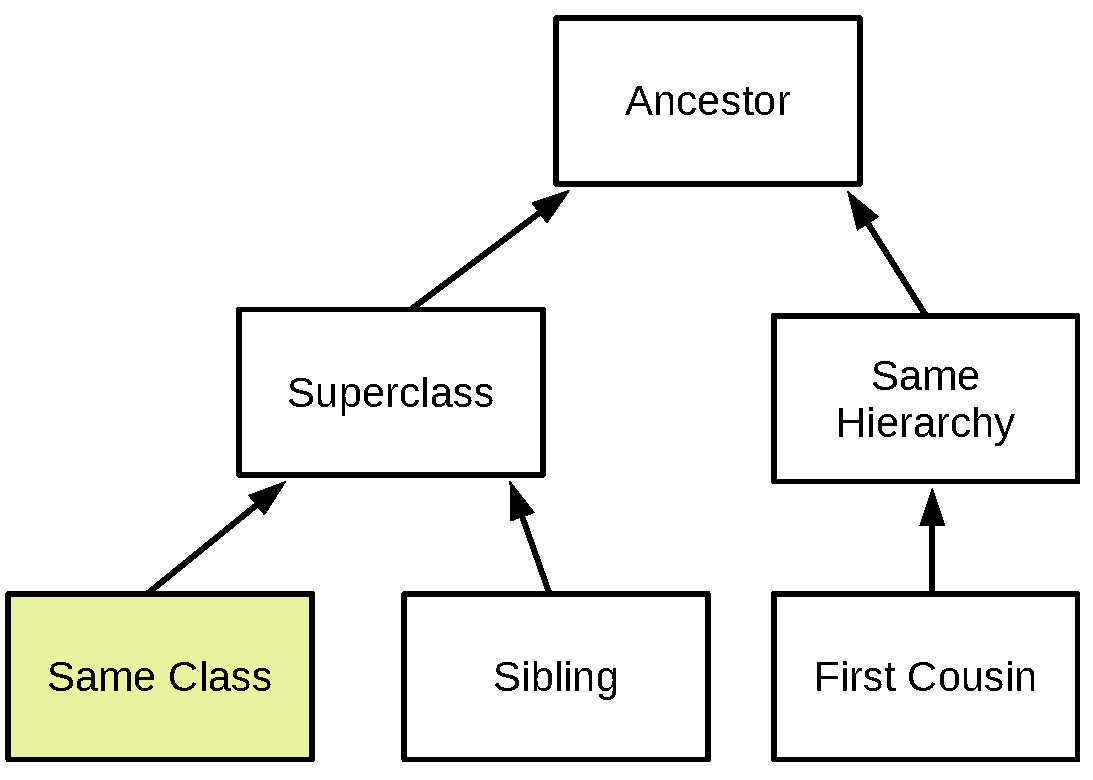
\includegraphics[width=1\columnwidth]{img/Relation}
  \caption{Abstract figure displaying some relations of clone classes. Arrows represent superclass relations.}
  \label{fig:clonerelation}
\end{figure}
Please note that none of these categories allow external classes (except for ``same external superclass''). So if two clone instances are related through external classes but do not share a common external superclass, it will be flagged as ``unrelated''. The main reason for this is that it is (often) not possible to refactor to external classes.

\subsubsection{Our setup}\label{chap:oursetup}
We use a similar setup to that used by Fontana et al. (Table~3 of Fontana et al. \cite{fontana2015duplicated}). Fontana et al. measure clones using their own tool (DCRA). As explained in section~\ref{ch:tool-overview}, we chose to implement our own tool, CloneRefactor. Therefore, the setup for our measurements differs as follows from Fontana et al.:
\begin{itemize}
  \item We consider clone classes rather than clone pairs. The rationale for this is given in section \ref{chap:cloneclasses}.
\item We use different thresholds regarding when a clone should be considered. Fontana et al. seek clones that span a minimum of 7 source lines of code (SLOC). We seek clones with a minimum size of 6 statements/declarations. This is explained detail in section \ref{chap:thresholds}.
\item We seek duplicates by statement/declaration rather than SLOC. This makes our analysis depend less on the coding style (in terms of newline usage) of the author of the software project.
\item We test a broader range of projects. Fontana et al. use a set of 50 relatively large projects. We use the corpus as explained in \ref{chap:corpus}, which contains a diverse set of projects (diverse both in volume and code quality).
\end{itemize}

\subsubsection{Our results} \label{chap:ourmeasurements}
Table~\ref{table:relations} contains our results regarding the relations between clone instances.

\begin{table}[H]
  \begin{center}
  \caption{Clone relations} \label{table:relations}
  \bigskip
\begin{tabular}{|l|l|l|} \hline
\textbf{Relation}  & \textbf{Amount} & \textbf{Percentage} \\ \hline
Unrelated          & 13,529           & 39.37               \\ \hline
Same Class          & 8,341            & 24.28               \\ \hline
Sibling            & 5,978            & 17.40               \\ \hline
Same Method         & 2,456            & 7.15                \\ \hline
External Superclass & 2,402            & 6.99                \\ \hline
First Cousin        & 695             & 2.02                \\ \hline
Superclass         & 489             & 1.42                \\ \hline
Common Hierarchy    & 442             & 1.29                \\ \hline
Ancestor           & 28              & 0.08               \\ \hline
\end{tabular}
\end{center}
\end{table}

The most notable difference when comparing it to the results of Fontana et al. \cite{fontana2015duplicated} is that in our results 39.37\% of clone are unrelated, while for them it was only 15.70\%. This might be due to the fact that we consider clone classes rather than clone pairs, and mark the clone class ``Unrelated'' even if just one of the clone instances is outside a hierarchy. It could also be that the corpus which we use, as it has generally smaller projects, uses more classes from outside the project (which are marked ``Unrelated'' if they do not have a common external superclass). About a fourth of all clone classes have all instances in the same class, which is generally easy to refactor. On the third place come the ``Sibling'' clones, which can often be refactored using a pull-up refactoring.

\subsection{Clone instance location}\label{chap:clonelocation}
After mapping the relations between individual clones, we looked at the location of individual clone instances. A paper by Lozano et al. \cite{lozano2007evaluating} discusses the harmfulness of cloning. The authors argue that 98\% are produced at method-level. However, this claim is based on a small dataset and based on human copy-paste behavior rather than static code analysis. We validated this claim over our corpus. The results for the clone instance locations are shown in table \ref{table:locations}. We chose the following categories:
\begin{enumerate}
  \item \textbf{Method/Constructor Level:} A clone instance that does not exceed the boundaries of a single method or constructor (optionally including the declaration of the method or constructor itself).
  \item \textbf{Class Level:} A clone instance in a class, that exceeds the boundaries of a single method or contains something else in the class (like field declarations, other methods, etc.).
  \item \textbf{Interface Level:} A clone that is (a part of) an interface.
  \item \textbf{Enumeration Level:} A clone that is (a part of) an enumeration.
\end{enumerate}

\begin{table}[H]
  \begin{center}
  \caption{Clone instance locations} \label{table:locations}
  \bigskip
\begin{tabular}{|l|l|l|}
\hline
\textbf{Location}  & \textbf{Amount}  & \textbf{Percentage} \\ \hline
Method Level       & 19,818           & 57.68               \\ \hline
Class Level        & 13,259           & 38.59               \\ \hline
Constructor Level  & 1,099            & 3.20                \\ \hline
Interface Level    & 110              & 0.32                \\ \hline
Enum Level         & 74               & 0.22                \\ \hline
\end{tabular}
\end{center}
\end{table}

Our results indicate that around 58\% of the clones are produced at method-level. About 39\% of clones either span several methods/constructors or contain something like a field declaration. Another 3\% of the clones are found in constructors. The amount of clones found in interfaces and enumerations is very low.

\subsection{Clone instance contents}\label{chap:clonecontents}
Finally, we looked at the contents of individual clone instances: what kind of declarations and statements do they span. We selected the following categories to be relevant for refactoring:
\begin{enumerate}
  \item \textbf{Full Method/Class/Interface/Enumeration:} A clone that spans a full class, method, constructor, interface or enumeration, including its declaration.
  \item \textbf{Partial Method/Constructor:} A clone that spans a method partially, optionally including its declaration.
  \item \textbf{Several Methods:} A clone that spans over two or more methods, either fully or partially, but does not span anything but methods (so not fields or anything in between).
  \item \textbf{Only Fields:} A clone that spans only global variables.
  \item \textbf{Includes Fields/Constructor:} A clone that spans a combination of fields and other things, like methods.
  \item \textbf{Method/Class/Interface/Enumeration Declaration:} A clone that contains the declaration (usually the first line) of a class, method, interface or enumeration.
  \item \textbf{Other:} Anything that does not match with above-stated categories.
\end{enumerate}

The results for these categories are displayed in table \ref{table:contents}.

\begin{table}[H]
  \begin{center}
  \caption{Clone instance contents} \label{table:contents}
  \bigskip
\begin{tabular}{|l|l|l|}
  \hline
  \textbf{Contents}                                                        & \textbf{Amount} & \textbf{Percentage} \\ \hline
  Partial Method                                                           & 19,264          & 56.07               \\ \hline
  Several Methods                                                          & 9,076           & 26.41               \\ \hline
  Includes Constructor                                                     & 1,528           & 4.45                \\ \hline
  Includes Field                                                           & 1,149           & 3.34                \\ \hline
  Partial Constructor                                                      & 1,098           & 3.20                \\ \hline
  Only Fields                                                              & 565             & 1.64                \\ \hline
  Full Method                                                              & 554             & 1.61                \\ \hline
  \begin{tabular}[c]{@{}l@{}}Includes Class\\ Declaration\end{tabular}     & 445             & 1.30                \\ \hline
  Other                                                                    & 369             & 1.07                \\ \hline
  Full Class                                                               & 192             & 0.56                \\ \hline
  \begin{tabular}[c]{@{}l@{}}Includes Enum\\ Constant\end{tabular}         & 52              & 0.15                \\ \hline
  \begin{tabular}[c]{@{}l@{}}Includes Enum\\ Declaration\end{tabular}      & 47              & 0.14                \\ \hline
  \begin{tabular}[c]{@{}l@{}}Includes Interface\\ Declaration\end{tabular} & 10              & 0.03                \\ \hline
  Full Interface                                                           & 6               & 0.02                \\ \hline
  Full Enumeration                                                         & 4               & 0.01                \\ \hline
\end{tabular}
\end{center}
\end{table}

Unsurprisingly, most clones span a part of a method. Just 1.6\% of the methods are cloned fully. More than a quarter of the clones spans over several methods, which makes extracting methods won't work in a case where a clone spans over several methods. About 4.5\% of clones include a constructor. About 3.3\% of clones include a global variable defined in a class.

\section{Merging duplicate code through refactoring}\label{chap:mergingdups}
Now we have mapped the contexts in which clones occur, we can start looking at refactoring opportunities. Regarding refactoring, we separate clones in two categories: easy and difficult refactoring opportunities. Easy refactoring opportunities are clones that can easily be automatically refactored. Examples of these opportunities are fully cloned methods or a set of fully cloned statements. According to the relation between the clone instances, we can propose a refactoring automatically.

However, a clone is not always easily merged. Sometimes a clone spans a statement partially (like a for-loop of which only it's declaration and a part of the body is cloned). Merging the clones can be harder in such instances. Also, the cloned code can contain statements like labels, return, break, continue, etc. In such instances, more conditions may apply to be able to conduct a refactoring, if advisable at all.

The most trivial way to merge a clone is through method extraction. However, method extraction is not always possible. For instance, if a part of a subtree (in a programs' AST) is matched as a clone. Because of this, we chose to measure what percentage of ``Partial Method'' clones are refactorable using method extraction. Our results are displayed in table \ref{table:refactorability}.

\begin{table}[H]
  \begin{center}
  \caption{Clone instance contents} \label{table:refactorability}
  \bigskip
\begin{tabular}{|l|l|l|}
\hline
\textbf{Refactorability}        & \textbf{Amount} & \textbf{Percentage} \\ \hline
\begin{tabular}[c]{@{}l@{}}Cannot directly\\be extracted\end{tabular}    & 10,990           & 41.91               \\ \hline
\begin{tabular}[c]{@{}l@{}}Is not a\\partial method\end{tabular} & 9,444            & 36.01               \\ \hline
\begin{tabular}[c]{@{}l@{}}Can be\\extracted\end{tabular}                & 5,791            & 22.08               \\ \hline

\end{tabular}
\end{center}
\end{table}

From this table, we can see that approximately 22 percent of the clones can be refactored through method extraction. For the other clones, we must first build a catalog of appropriate refactorings.

\section{Threats to validity}\label{chap:threatstovalidity}
We noticed that, when measuring over a corpus of this size, the thresholds that we use for the clone detection have a big impact on the results. There does not seem to be one golden set of thresholds, some thresholds work in some situations but fail in others. We have chosen thresholds that, according to our manual assessment, seemed optimal. However, by using these, we definitely miss some harmful clones.

Another thread to validity is that currently, in a very small number of cases, clone detection might result in a false positive. This is in cases where two lines are equal, but they actually call different methods with the same method signature. In such a case, merging such clones might turn out to change the functionality of the program. Solving this problem is one of our next steps in this research.

\section{Conclusion and next steps}\label{chap:conclusion}
In the research we have conducted so far we have made three novel contributions:
\begin{itemize}
    \item We proposed a method in which we can detect clones that can/should be refactored.
    \item We mapped the context of clones in a large corpus of open source systems.
    \item We mapped the opportunities to perform method extraction on clones in a large corpus of open source systems.
\end{itemize}

We have into existing definitions for different types of clones \cite{roy2007survey} and proposed solutions for problems that these types have with regards to automated refactoring. We propose that fully qualified identifiers of method call signatures and type references should be considered instead of their plain text representation. Furthermore, we should define thresholds for variability in variables, literals and method calls, in order to limit the number of parameters that the merged unit shall have.

The research that we have conducted so far analyzes the context of different kinds of clones and prioritizes their refactoring. Firstly, we looked at the inheritance relation of clone instances in a clone class. We have found that more than a third of all clone classes are flagged unrelated, which means that they have at least one instance that has no relation through inheritance with the other instances. For about a fourth of the clone classes all of its instances are in the same class. For about a sixth of the clone classes have clone instances that are siblings of each other (share the same superclass).

Secondly, we looked at the location of clone instances. Most clone instances are found at method level, about 58 percent. About 39 percent of clone instances were found at class level. We defined ``class level clones'' as clones that exceed the boundaries of a single method or contain something else in the class (like field declarations, other methods, etc.). Thirdly, we looked at the contents of clone instances. Most clones span a part of a method (56 percent). About 26 percent of clones span over several methods. 

We also looked into the refactorability of clones that span a part of a method. Over 22 percent of the clones can directly be refactored by extracting them to a new method (and calling the method at all usages using their relation). The main reason that most clones that span a part of a method cannot directly be refactored by method extraction, is that they are nested in such a way that method extraction would leave side effects (for instance, we cannot extract half of a for-loop).

\subsection{Next steps}
The next step is to integrate our solutions for the problems related to clone types into our CloneRefactor tool. This way, we can perform our experiments for these novel clone definitions. We are curious to see how it compares with the results we had so far.

Furthermore, we want to start automatically refactoring clones. On basis of our initial results, we have determined that we can best start with the automatic refactoring of clones that can be extracted to a method. If this works, we can already decrease duplication by 22\%.

\section*{Acknowledgements}
We would like to thank the Software Improvement Group (SIG) for their continuous support in this project.

\bibliographystyle{alpha}
\bibliography{res}

\end{document}
